\begin{figure*}[p]
\centering
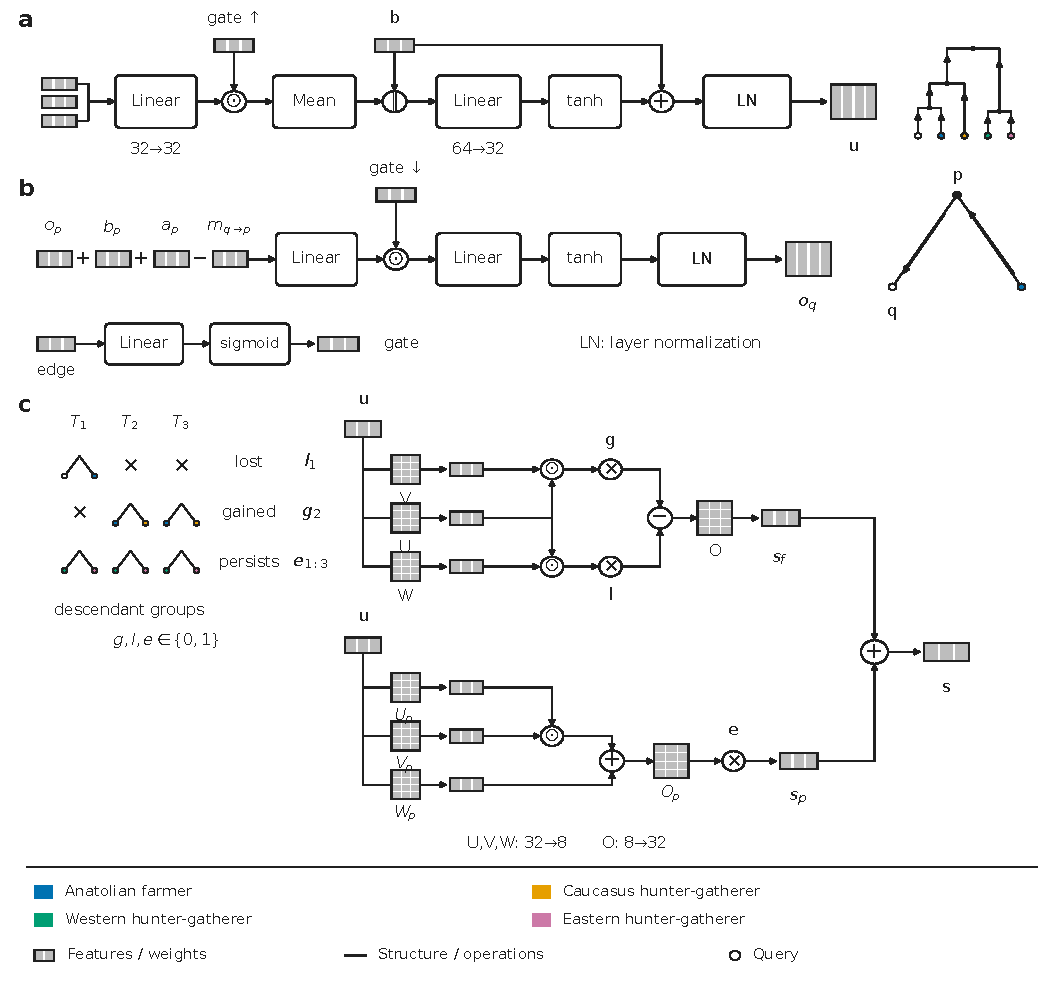
\includegraphics[width=\textwidth]{figures/TreeLoom_operators.pdf}
\caption{\textbf{a,} Upward update at one node. Each child state is transformed and gated before the arithmetic mean over children. This mean joins input $b$, followed by a linear map, tanh, residual addition and learned layer normalization. The operator repeats from leaves to root.
\textbf{b,} Downward update. Parent outside state $o_p$, input $b_p$ and mean child message $a_p$ are combined, excluding the recipient's normalized contribution $m_{q\to p}$. The displayed maps and edge gate give outside state $o_q$. The root starts at zero. Nine observed edge features produce separate directional gates.
\textbf{c,} Descendant pairs illustrate loss, gain and persistence across trees. Binary flags select factored transformations of the current upward state $u_v$, with separate weights for the two corrections. Neighboring hidden states do not enter these circuits. The symbol $\odot$ denotes elementwise product, Scale $\times$ multiplies a vector by a scalar, and $\parallel$ concatenates. Input signs define subtraction order. Diagram state $u$ is $h$ in the equations. Colors have the meanings shown in the legend.}
\label{fig:operators}
\end{figure*}
